In 1870, the Swiss chemist \emph{Miescher} discovered inside the nucleus of a cell a giant molecule: \textbf{deoxyribonucleic acid}. 
\\
\\In 1953, two biochemists, the American \emph{James Watson} and the English \emph{Francis Crick} show that the structure of the DNA molecule is comparable to that of a spiral staircase; a sort of spiral-shaped double helix.
\\
\\
\\	
\textbf{Deoxyribonucleic acid (DNA)} is a molecule that encodes the genetic instructions used in the development and functioning of all known living organisms and many vi-ruses. DNA is a nucleic acid; together with proteins and carbohydrates, nucleic acids compose the three major macromolecules essential for all known forms of life.
\\
\\Most DNA molecules consist of \emph{two biopolymer strands coiled around each other to form a double helix}. The two DNA strands are known as polynucleotides since they are composed of simpler units called nucleotides. Each nucleotide is composed of a \textbf{nitrogen-containing nucleobase}—either \textbf{guanine} (G), \textbf{adenine} (A), \textbf{thymine} (T), or \textbf{cytosine} (C)—as well as a monosaccharide sugar called \textbf{deoxyribose} and a \textbf{phosphate} group. The nucleotides are joined to one another in a chain by \emph{covalent bonds between the sugar of one nucleotide and the phosphate of the next}, resulting in an \emph{alternating sugar-phosphate backbone}. According to base pairing rules (A with T and C with G), hydrogen bonds bind the nitrogenous bases of the two separate polynucleotide strands to make double-stranded DNA.

\begin{figure}[ht!]
	\centering
	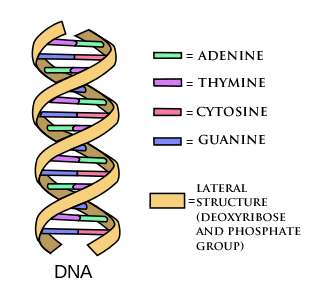
\includegraphics[width=90mm]{../Images/DNA_double_helix.png}
	\label{overflow}
	\caption{DNA structure}
	\end{figure}

DNA is \textbf{well-suited for biological information storage}. The DNA backbone is resistant to cleavage, and both strands of the double-stranded structure store the same biological information. Biological information is \textbf{replicated} as the two strands are sepa-rated. A significant portion of DNA (more than 98 per cent for humans) is non-coding, meaning that these sections do not serve a function of encoding proteins.
\\
\\
\\That said, it is easy to understand how DNA is important for life. For this reason, even a small mutation (a change of the nucleotide sequence of the genome of an or-ganism) can be decisive and cause diseases.
\\
\\In this essay we will discuss a particular case of genomic mutation, the \textbf{Single Nucleotide Polymorphism}.